\documentclass{article}

\usepackage{amssymb}
\usepackage{tikz}
\usetikzlibrary{positioning}
\usepackage{ stmaryrd }

\title{Interaction Diagram - Rate Book}
\author{Steve Monson}

% no page number at bottom
\pagenumbering{gobble}

\begin{document}
\maketitle

\begin{center}
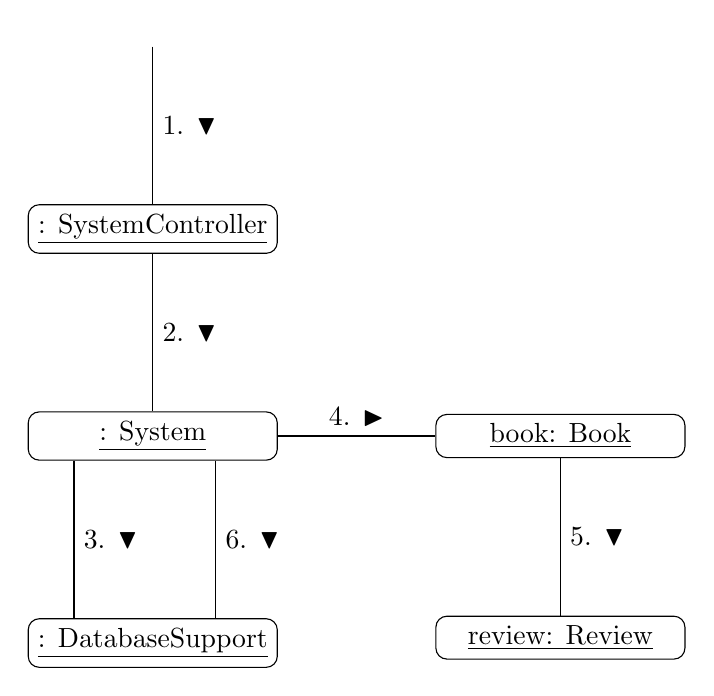
\begin{tikzpicture}[
  auto,
  block/.style = {
    minimum width = 9em,
    rectangle,
    draw=black,
    align=center,
    rounded corners
  }
]

% Content goes here
\node[] (start)  {};

\node[block, below = 2cm of start]      (controller) {\underline{: SystemController}};
\node[block, below = 2cm of controller] (system)     {\underline{: System}}; 
\node[block, below = 2cm of system]     (database)   {\underline{: DatabaseSupport}};
\node[block, right = 2cm of system]       (book)       {\underline{book: Book}};
\node[block, below = 2cm of book]       (review)    {\underline{review: Review}};

\draw (start)      -- (controller) node[midway] {1. $\blacktriangledown$};
\draw (controller) -- (system)     node[midway] {2. $\blacktriangledown$};
\draw ([xshift=-1cm]system.south) -- ([xshift=-1cm]database.north)
      node[midway] {3. $\blacktriangledown$};
\draw (system)     -- (book)       node[midway] {4. $\blacktriangleright$};
\draw (book)    -- (review)        node[midway] {5. $\blacktriangledown$};
\draw ([xshift=0.8cm]system.south) -- ([xshift=0.8cm]database.north)
      node[midway] {6. $\blacktriangledown$};

\end{tikzpicture}
\end{center}

\vspace{0.5cm}

\begin{enumerate}
    \item \texttt{b:= addRating(uid:String, bid:String, rating:int):boolean}
    \item \texttt{b:= addRating(uid:String, bid:String, rating:int):boolean}
    \item \texttt{b:= getBook(bid:String):Book}
    \item \texttt{b:= addRating(rating:int):boolean}
    \item \texttt{Create()}
    \item \texttt{b:= putBook(book:Book):boolean}
\end{enumerate}

\end{document}
